% Measurement results / analysis / discussion:
% whatever you have done, you must comment it, compare it to other systems, evaluate it
% usually, adequate graphs help to show the benefits of your approach
% caution: each result/graph must be discussed! what’s the reason for this peak or why have you ovserved this effect

\chapter{Evaluation}\label{ch:evaluation}\glsresetall
TBW
\section{Experimental Setup}
Evaluation of our system solely depends on how the deep learning mode perform with the datasets we generated. We retrieved real-time data from $138$ different markets over a period of $33$ days, and the pairing coin of each market is Bitcoin. The data retriever fetched data in a fixed interval of $5$ seconds, resulting approximately $\numprint{570 000}$ samples per market. In total we collected \SI{47}{\giga\byte} of data. We processed the data, and the time lag we choose when calulcating the percentage of change was $10$ minutes, or approximaltely 120 points.

% 280 anomalies
% 200 pd

The computer we used to train our model with has the following scpecifications:
\begin{itemize}
    \item CPU - Intel Xeon E5-1620 \SI{3.9}{\giga\hertz}
    \item RAM - \SI{64}{\mebi\byte} DDR3 
    \item GPU - Nvidia GeForce GTX 770
\end{itemize}

We used the anomaly detection algorithm as we have previously outlined to detect anomalies from Binance, and filtered out the all anomalies that looked like a \ac{pd}. The following charts shows some of intervals that where labeled.

\begin{figure}
    \centering
    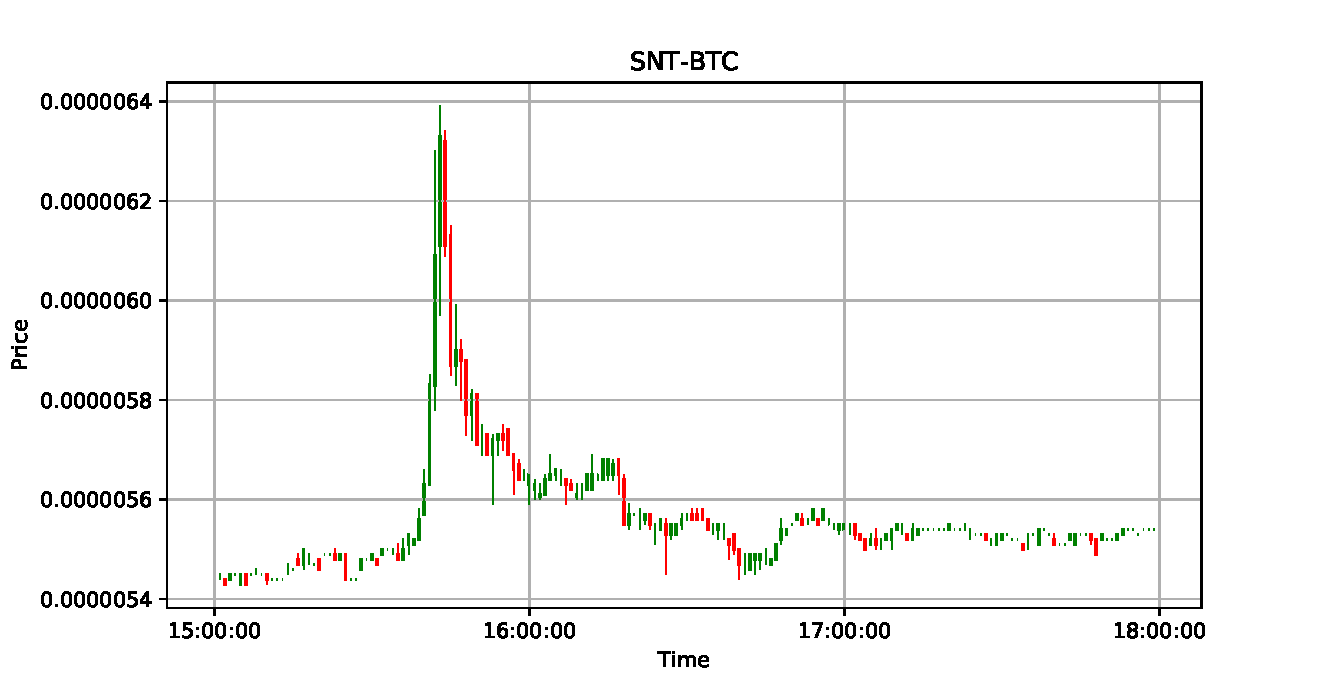
\includegraphics[width=\textwidth]{true_1.pdf}
    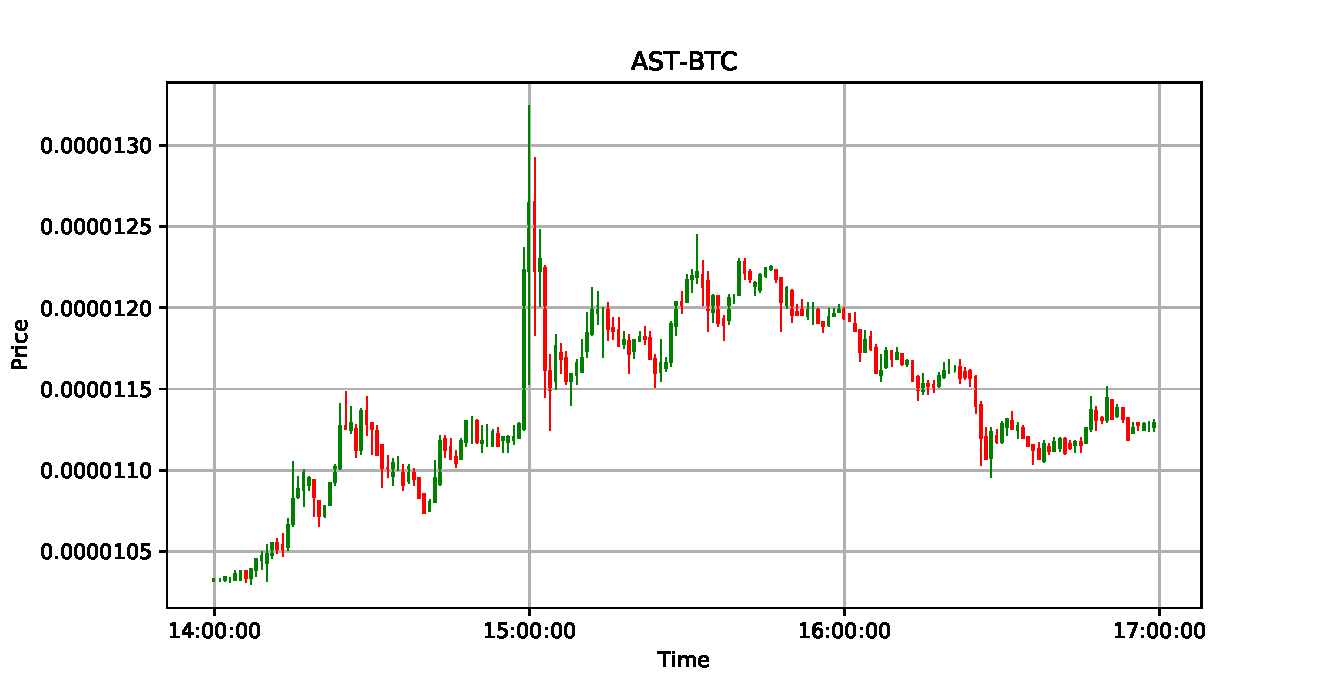
\includegraphics[width=\textwidth]{true_2.pdf}
    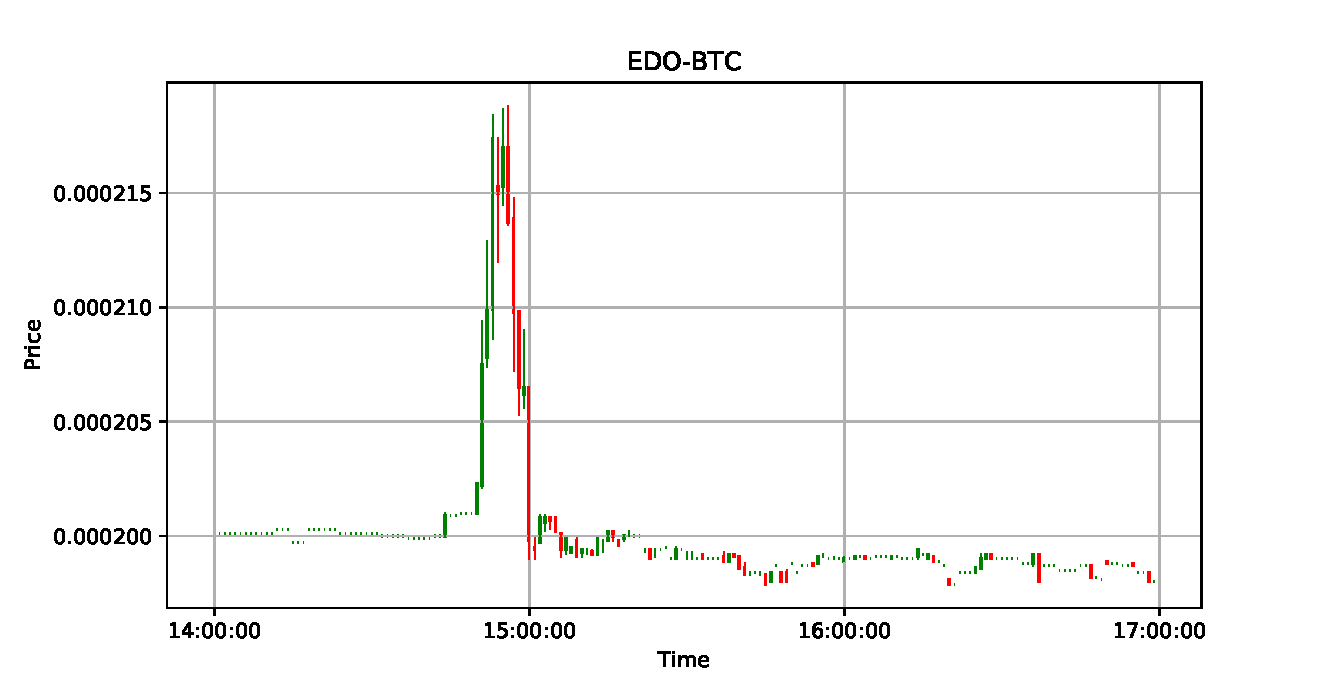
\includegraphics[width=\textwidth]{true_3.pdf}
    \caption{Anomalies that seems like a \ac{pd}}
    \label{fig:label_true}
\end{figure}

\begin{figure}
    \centering
    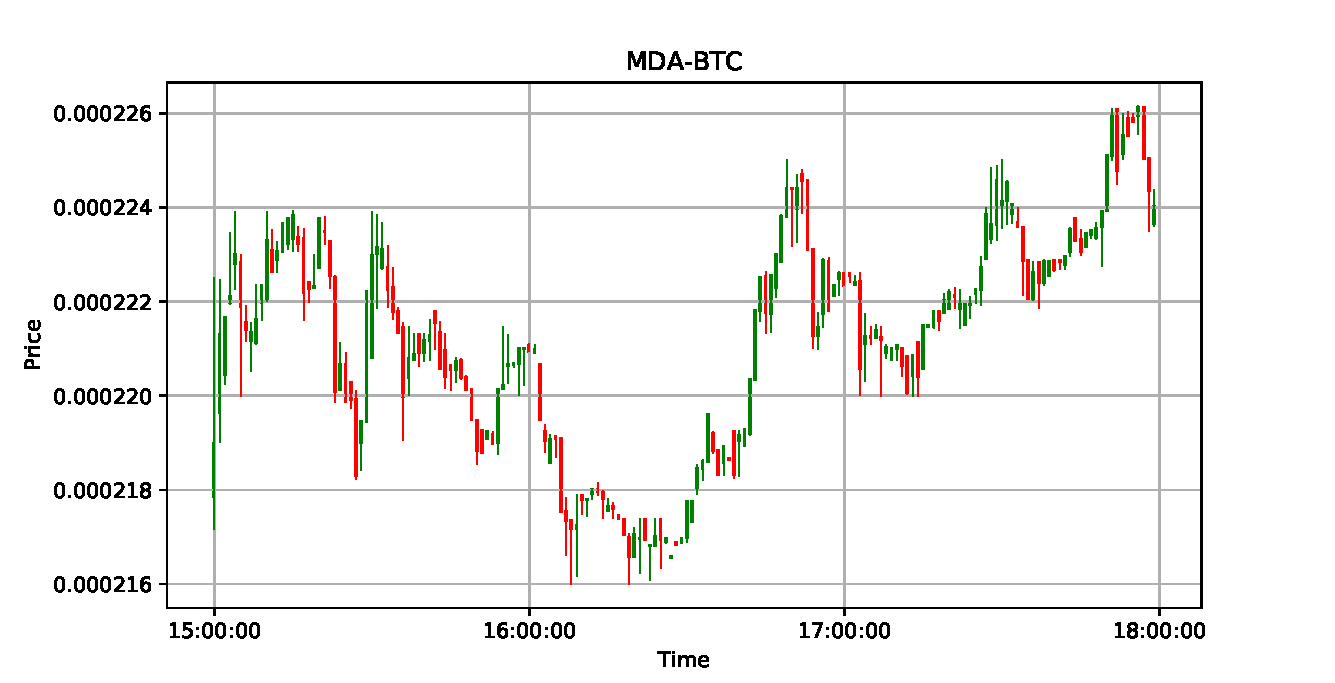
\includegraphics[width=\textwidth]{false_1.pdf}
    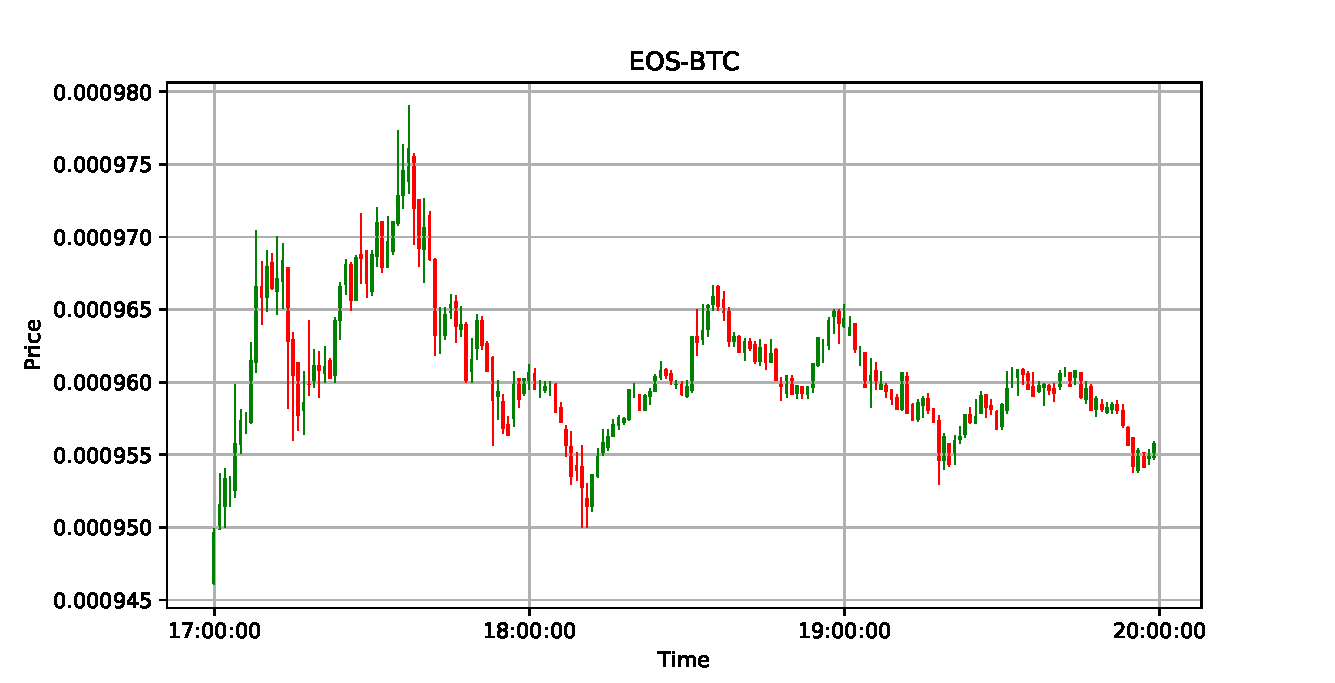
\includegraphics[width=\textwidth]{false_2.pdf}
    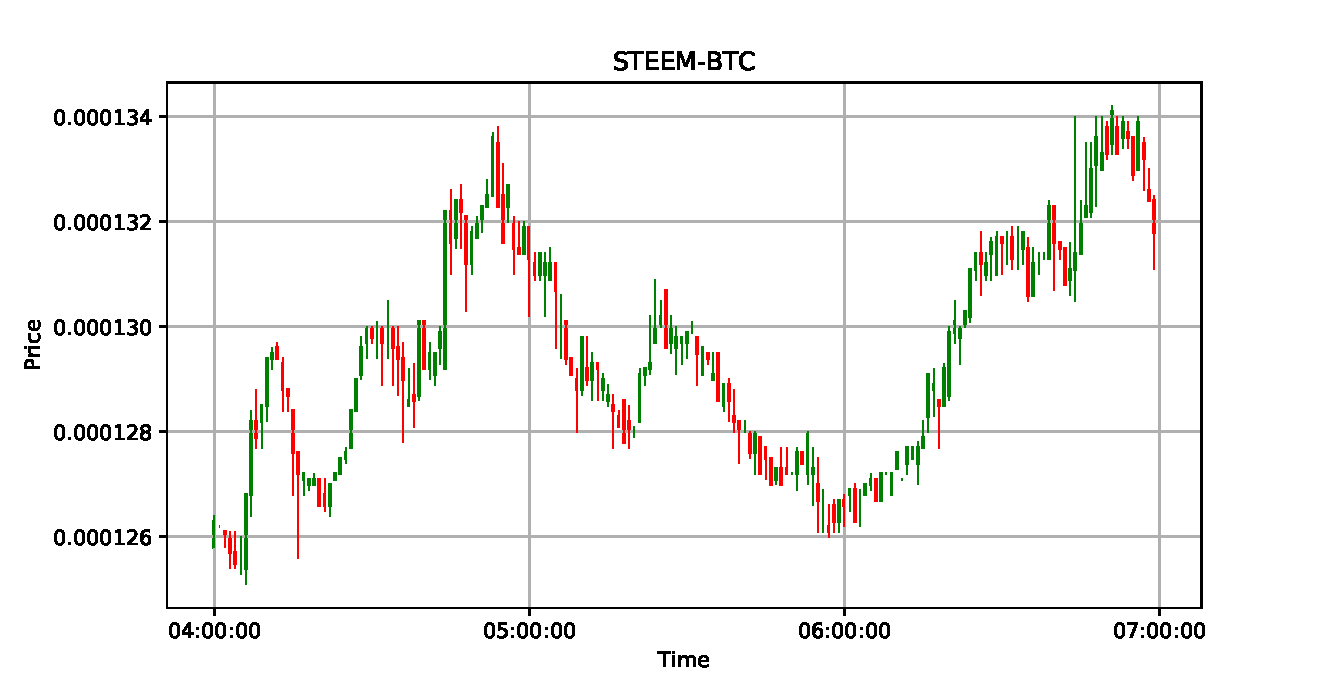
\includegraphics[width=\textwidth]{false_3.pdf}
    \caption{Anomalies that not seems like a \ac{pd}}
    \label{fig:label_false}
\end{figure}

We choose to split our dataset into a training and test set, where the training set takes up $75\%$ ($104$ markets), and the test consists of the remaining $25\%$ ($33$ markets) of the dataset.  With the training dataset that we generated, we undersampled the dataset to create a blanaced dataset to trained a \ac{lstm} network with, where the hidden layer contain a single layer with $50$ \ac{lstm} cells, we also added dropout the \ac{lstm} cells, to prevent over-fitting as \ac{lstm} tends to often overfit their training data~\cite{overfit}. The output layer contained a single perceptron. We trained the network with balanced dataset in  $\numprint{5000}$ epochs. Also, we use the \emph{adam} optimizer, which is an extension to stochastic gradient descent~\cite{kingma2014adam}, the optimizer has shown that the model's weights will converge faster that results in great performance rapidly~\cite{adam}. To classify the performance of the model, we classified all samples in the test dataset.

\section{Results}
We evaluate our model by using several metrics, the first metric we use is a confusion matrix like \autoref{tab:confmat}. A confusion matrix shows the number of correct and incorrect classifies samples. \autoref{tab:model_performance} shows the results we obtained by using the parameters described. With the confusion matrix we can define a various performance measures as \autoref{tab:performance} illustrates.

\begin{table}
    \centering
    \begin{tabular}{|c|c|c|c|}\hline
                &   \multicolumn{3}{c|}{Predicted class}\\\hline
    True class  &  Positive             & Negative              & Total \\\hline
    Positive    & $tp$: true positive   & $fn$: false negative  & $p$   \\
    Negative    & $fp$: false positive  & $tn$: true negative   & $n$   \\\hline
    Total       & $p'$                  & $n'$                  & $N$   \\\hline
    \end{tabular}
    \caption{Confusion matrix}
    \label{tab:confmat}
\end{table}
\begin{table}
        \centering
        \begin{tabularx}{\textwidth}{ |R|R|R|R| }\hline
                    &   \multicolumn{3}{c|}{Predicted class}\\\hline
        True class  & Positive              & Negative              & Total                 \\\hline
        Positive    & $\numprint{7910}$     & $\numprint{911}$      & $\numprint{8821}$     \\
        Negative    & $\numprint{388795}$   & $\numprint{17933021}$ & $\numprint{18321816}$ \\\hline
        Total       & $\numprint{396705}$   & $\numprint{17933932}$ & $\numprint{18330637}$ \\\hline
        \end{tabularx}
        \caption{\project's confusion matrix}
        \label{tab:model_performance}
\end{table}
\begin{table}
    \centering
    \begin{tabular}{|c|c|r|}\hline
    Name        & Formula       &   Result      \\\hline
    error       & $(fp+fn)/N$   &   $0.0217$    \\
    accuracy    & $(tp+tn)/N$   &   $0.9782$    \\\hline
    tp-rate     & $tp/p$        &   $0.8967$    \\
    fp-rate     & $fp/n$        &   $0.0212$    \\\hline
    sensitivity & $tp/p$        &   $0.8967$    \\
    specificity & $tn/n$        &   $0.9787$    \\\hline
    recall      & $tp/p$        &   $0.8967$    \\
    precision   & $tp/p'$       &   $0.0199$    \\\hline
    \end{tabular}
    \caption{Performance measure}
    \label{tab:performance}
\end{table}

From \autoref{tab:performance}, we can see that the model itself achieve a respective accuracy, in total it achieve around $98\%$ accuracy. The true positive rate is approximately $90\%$ and true negative ratio is circa $98\%$. These ratios is in general are good, if and only if the problem itself is hard to solve and if the dataset is balanced. Detecting \ac{pd} is a hard problem, it is hard even for us to identify \acp{pd}, there was multiple occasions during the filtering phase where we had problems with distinguishing \acp{pd}. Also, considering the type of data we had to work with, and how few \acp{pd} samples we have compared to regular trading data, there was over $\numprint{2000}$ times more samples that is categorized as negative than positive,....

In terms of \emph{specificity}, the model almost scores flawlessly, $99.99\%$. Specificity is ratio of how often we not classifies a positive \ac{pd} as negative. From the \autoref{tab:confmat}, we see that the model classified $911$ positive points as negative, while we classified $\numprint{17933021}$ correctly negative. Hence, the model is very precise when it boils down to classify negative samples as negative.

\autoref{fig:roc} illustrate the \ac{roc} curve of our model, and it gives us a visual perspective of the performance of the model. Ideally, a classifier has a tp-rate of $1$ and an fp-rate of $0$, and hence a classifier is better the more its \ac{roc} curve gets closer to the upper-left corner. On the diagonal, we make as many true decisions as false ones, and this is the worst case~\cite[p.~563]{alpaydin2014introduction}. Our \ac{roc} curve also shows that our model has accurate predictable capabilities. The \ac{auc} score represents the probability that a randomly chosen positive example is correctly classified ranked with greater suspicion than a randomly chosen negative example~\cite{bradley1997use}.
\begin{figure}[ht]
    \centering
    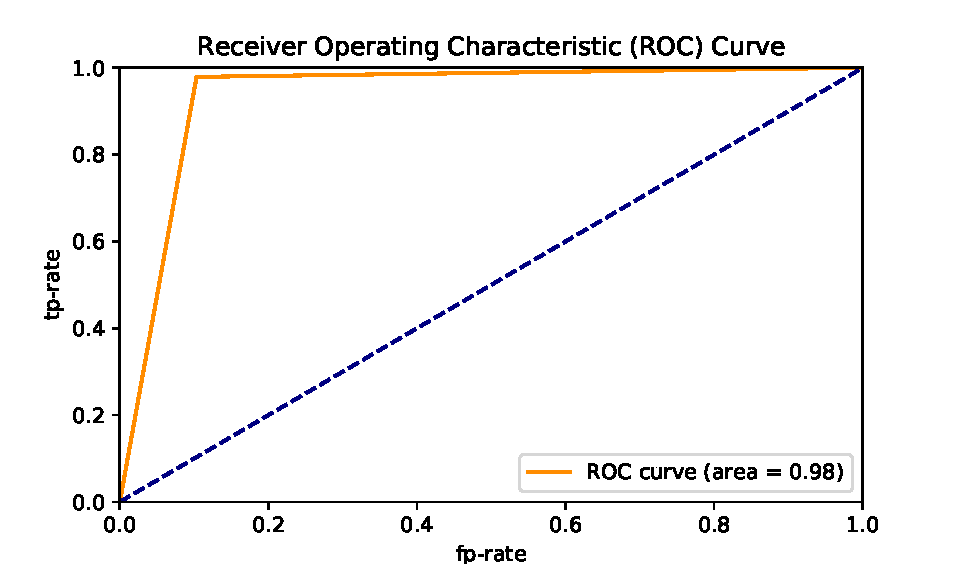
\includegraphics[width=\textwidth]{results/roc.pdf}
    \caption{Roc Curve}
    \label{fig:roc}
\end{figure} 

Currently, some metrics clearly shows that the model has good predictable capabilities in terms of accuracy. Another metric that reveal  the weakness of our model, is the f-score. As the \ac{roc} curve focuses on the relationship between tp-rate and fp-rate, the f-score measure our model test's accuracy with the weight on the measures \emph{recall} and \emph{precision}. Precision is an important measure when it comes to imbalanced dataset because the precision says something regarding the accuracy of correctly classified positive predicted samples. Our model only achieve a disappointing precision on $2\%$, and that value clearly demonstrate that $2\%$ of the samples that we classify as \acp{pd} truly are \acp{pd}, and regarding the f-score. An ideal f-score is $1$, and the worst is $0$. This measure is flexible in terms that we can weigh both recall and precision differently by adjusting the parameter $\gamma$. Where the closer $\gamma$ is to $0$, the more we weigh precision, when $\gamma$ is $1$ we wight them equally, and finally when $\gamma$ is over $1$, we weigh recall most.
\begin{align}\label{eq:f_score}
    F_\beta &= (1+\beta^2) \cdot \frac{\text{precision} \cdot \text{recall}}{(\beta^2\cdot\text{precision}) + \text{recall}},\quad
    \begin{cases} 
    F_{0.5} &= 0.0247\\ 
    F_1     &= 0.0389\\ 
    F_2     &= 0.0912\\ 
    \end{cases}
\end{align}

The following results shows the confusion matrix of each classified market.

\begin{table}[H]
        \centering
        \begin{tabularx}{\textwidth}{ |R|R||R|R||R|R| }
                \multicolumn{2}{c}{WABI-BTC} & \multicolumn{2}{c}{MITH-BTC} & \multicolumn{2}{c}{ETH-BTC} \\\hline
                $\numprint{376}$\cellcolor{green!91} & $\numprint{36}$\cellcolor{red!9} & $\numprint{0}$\cellcolor{green!0} & $\numprint{2}$\cellcolor{red!100} & $\numprint{0}$\cellcolor{green!100} & $\numprint{0}$\cellcolor{red!0} \\
                $\numprint{23440}$\cellcolor{red!5} & $\numprint{531622}$\cellcolor{green!95} & $\numprint{26798}$\cellcolor{red!5} & $\numprint{528675}$\cellcolor{green!95} & $\numprint{0}$\cellcolor{red!0} & $\numprint{555474}$\cellcolor{green!100} \\
                \hline
                \addlinespace[.2cm]

                \multicolumn{2}{c}{XRP-BTC} & \multicolumn{2}{c}{BTT-BTC} & \multicolumn{2}{c}{OST-BTC} \\\hline               
                $\numprint{0}$\cellcolor{green!100} & $\numprint{0}$\cellcolor{red!0} & $\numprint{0}$\cellcolor{green!100} & $\numprint{0}$\cellcolor{red!0} & $\numprint{488}$\cellcolor{green!90} & $\numprint{53}$\cellcolor{red!10} \\
                $\numprint{0}$\cellcolor{red!0} & $\numprint{555474}$\cellcolor{green!100} & $\numprint{3400}$\cellcolor{red!1} & $\numprint{552074}$\cellcolor{green!99} & $\numprint{8705}$\cellcolor{red!2} & $\numprint{546228}$\cellcolor{green!98} \\
                \hline
                \addlinespace[.2cm]

                \multicolumn{2}{c}{CDT-BTC} & \multicolumn{2}{c}{GNT-BTC} & \multicolumn{2}{c}{TRX-BTC} \\\hline               
                $\numprint{407}$\cellcolor{green!88} & $\numprint{51}$\cellcolor{red!12} & $\numprint{375}$\cellcolor{green!78} & $\numprint{105}$\cellcolor{red!22} & $\numprint{0}$\cellcolor{green!100} & $\numprint{0}$\cellcolor{red!0} \\
                $\numprint{18303}$\cellcolor{red!4} & $\numprint{536713}$\cellcolor{green!96} & $\numprint{20994}$\cellcolor{red!4} & $\numprint{534000}$\cellcolor{green!96} & $\numprint{289}$\cellcolor{red!1} & $\numprint{555185}$\cellcolor{green!99} \\
                \hline
                \addlinespace[.2cm]

                \multicolumn{2}{c}{MTH-BTC} & \multicolumn{2}{c}{DLT-BTC} & \multicolumn{2}{c}{SC-BTC} \\\hline                
                $\numprint{487}$\cellcolor{green!97} & $\numprint{16}$\cellcolor{red!3} & $\numprint{584}$\cellcolor{green!87} & $\numprint{85}$\cellcolor{red!13} & $\numprint{0}$\cellcolor{green!100} & $\numprint{0}$\cellcolor{red!0} \\
                $\numprint{12032}$\cellcolor{red!3} & $\numprint{542939}$\cellcolor{green!97} & $\numprint{19223}$\cellcolor{red!3} & $\numprint{535580}$\cellcolor{green!97} & $\numprint{7234}$\cellcolor{red!2} & $\numprint{548240}$\cellcolor{green!98} \\
                \hline
                \addlinespace[.2cm]

                \multicolumn{2}{c}{SNT-BTC} & \multicolumn{2}{c}{XEM-BTC} & \multicolumn{2}{c}{VIB-BTC} \\\hline                
                $\numprint{323}$\cellcolor{green!88} & $\numprint{40}$\cellcolor{red!12} & $\numprint{0}$\cellcolor{green!100} & $\numprint{0}$\cellcolor{red!0} & $\numprint{674}$\cellcolor{green!99} & $\numprint{7}$\cellcolor{red!1} \\
                $\numprint{8138}$\cellcolor{red!2} & $\numprint{546973}$\cellcolor{green!99} & $\numprint{914}$\cellcolor{red!1} & $\numprint{554559}$\cellcolor{green!99} & $\numprint{22358}$\cellcolor{red!5} & $\numprint{532435}$\cellcolor{green!95} \\
                \hline
                \addlinespace[.2cm]

                \multicolumn{2}{c}{MTL-BTC} & \multicolumn{2}{c}{HC-BTC} & \multicolumn{2}{c}{STORM-BTC} \\\hline             
                $\numprint{477}$\cellcolor{green!93} & $\numprint{36}$\cellcolor{red!7} & $\numprint{251}$\cellcolor{green!57} & $\numprint{188}$\cellcolor{red!43} & $\numprint{0}$\cellcolor{green!100} & $\numprint{0}$\cellcolor{red!0} \\
                $\numprint{29687}$\cellcolor{red!6} & $\numprint{525274}$\cellcolor{green!94} & $\numprint{5213}$\cellcolor{red!1} & $\numprint{549822}$\cellcolor{green!99} & $\numprint{14995}$\cellcolor{red!3} & $\numprint{540479}$\cellcolor{green!97} \\
                \hline
                \addlinespace[.2cm]

                \multicolumn{2}{c}{INS-BTC} & \multicolumn{2}{c}{LUN-BTC} & \multicolumn{2}{c}{NXS-BTC} \\\hline               
                $\numprint{0}$\cellcolor{green!0} & $\numprint{1}$\cellcolor{red!100} & $\numprint{792}$\cellcolor{green!93} & $\numprint{57}$\cellcolor{red!7} & $\numprint{0}$\cellcolor{green!100} & $\numprint{0}$\cellcolor{red!0} \\
                $\numprint{7032}$\cellcolor{red!2} & $\numprint{548439}$\cellcolor{green!98} & $\numprint{12443}$\cellcolor{red!3} & $\numprint{542182}$\cellcolor{green!97} & $\numprint{6554}$\cellcolor{red!1} & $\numprint{548920}$\cellcolor{green!99} \\
                \hline
                \addlinespace[.2cm]

                \multicolumn{2}{c}{TNB-BTC} & \multicolumn{2}{c}{NPXS-BTC} & \multicolumn{2}{c}{ZRX-BTC} \\\hline               
                $\numprint{441}$\cellcolor{green!99} & $\numprint{3}$\cellcolor{red!1} & $\numprint{0}$\cellcolor{green!100} & $\numprint{0}$\cellcolor{red!0} & $\numprint{0}$\cellcolor{green!100} & $\numprint{0}$\cellcolor{red!0} \\
                $\numprint{47144}$\cellcolor{red!9} & $\numprint{507886}$\cellcolor{green!91} & $\numprint{3381}$\cellcolor{red!1} & $\numprint{552093}$\cellcolor{green!99} & $\numprint{10138}$\cellcolor{red!2} & $\numprint{545336}$\cellcolor{green!98} \\
                \hline
                \addlinespace[.2cm]

                \multicolumn{2}{c}{VET-BTC} & \multicolumn{2}{c}{RCN-BTC} & \multicolumn{2}{c}{ETC-BTC} \\\hline                
                $\numprint{0}$\cellcolor{green!100} & $\numprint{0}$\cellcolor{red!0} & $\numprint{487}$\cellcolor{green!95} & $\numprint{26}$\cellcolor{red!5} & $\numprint{160}$\cellcolor{green!84} & $\numprint{30}$\cellcolor{red!16} \\
                $\numprint{1321}$\cellcolor{red!2} & $\numprint{554153}$\cellcolor{green!98} & $\numprint{10697}$\cellcolor{red!2} & $\numprint{544264}$\cellcolor{green!98} & $\numprint{2890}$\cellcolor{red!1} & $\numprint{552394}$\cellcolor{green!99} \\
                \hline
                \addlinespace[.2cm]

                \multicolumn{2}{c}{SNM-BTC} & \multicolumn{2}{c}{SKY-BTC} & \multicolumn{2}{c}{LOOM-BTC} \\\hline              
                $\numprint{1209}$\cellcolor{green!95} & $\numprint{55}$\cellcolor{red!5} & $\numprint{141}$\cellcolor{green!76} & $\numprint{44}$\cellcolor{red!24} & $\numprint{0}$\cellcolor{green!100} & $\numprint{0}$\cellcolor{red!0} \\
                $\numprint{21950}$\cellcolor{red!4} & $\numprint{532260}$\cellcolor{green!96} & $\numprint{14423}$\cellcolor{red!2} & $\numprint{540866}$\cellcolor{green!98} & $\numprint{1485}$\cellcolor{red!1} & $\numprint{553989}$\cellcolor{green!99} \\
                \hline
                \addlinespace[.2cm]

                \multicolumn{2}{c}{CVC-BTC} & \multicolumn{2}{c}{PHX-BTC} & \multicolumn{2}{c}{PPT-BTC} \\\hline               
                $\numprint{238}$\cellcolor{green!76} & $\numprint{74}$\cellcolor{red!24} & $\numprint{0}$\cellcolor{green!0} & $\numprint{1}$\cellcolor{red!100} & $\numprint{0}$\cellcolor{green!0} & $\numprint{1}$\cellcolor{red!100} \\
                $\numprint{8393}$\cellcolor{red!1} & $\numprint{546769}$\cellcolor{green!99} & $\numprint{13211}$\cellcolor{red!2} & $\numprint{542262}$\cellcolor{green!98} & $\numprint{6010}$\cellcolor{red!1} & $\numprint{549463}$\cellcolor{green!99} \\
                \hline
        \end{tabularx}
        \caption[\project's confusion matrices of tested markets]{confusion matrices of the $33$ tested markets.}
        \label{tab:results}
\end{table}
\section{Discussion}